% !TEX program = xelatex
\documentclass[10pt,letterpaper,twocolumn]{article}

% === GEOMETRY ===
\usepackage[top=0.75in, bottom=0.75in, left=0.75in, right=0.75in]{geometry}

% === FONTS ===
\usepackage{fontspec}
\setmainfont{Latin Modern Roman}[
  Extension=.otf,
  UprightFont=lmroman10-regular,
  BoldFont=lmroman10-bold,
  ItalicFont=lmroman10-italic,
  BoldItalicFont=lmroman10-bolditalic,
]
\setsansfont{Latin Modern Sans}[
  Extension=.otf,
  UprightFont=lmsans10-regular,
  BoldFont=lmsans10-bold,
  ItalicFont=lmsans10-oblique,
  BoldItalicFont=lmsans10-boldoblique,
]
\setmonofont{Latin Modern Mono}[
  Extension=.otf,
  UprightFont=lmmono10-regular,
  ItalicFont=lmmono10-italic,
  Scale=0.85,
]
% YWFT Processing carries the display title only.
\newfontfamily\acbold{ywft-processing-bold}[Path=../../system/public/type/webfonts/,Extension=.ttf]

% === PACKAGES ===
\usepackage{xcolor}
\usepackage{titlesec}
\usepackage{enumitem}
\usepackage{tabularx}
\usepackage{colortbl}
\usepackage{hhline}
\usepackage{array}
\usepackage{fancyhdr}
\usepackage{hyperref}
\usepackage{xurl}
\usepackage{graphicx}
\usepackage{ragged2e}
\usepackage{microtype}
\usepackage{caption}
\usepackage{tikz}
\usepackage{../ac-source-bundle}

% === COLOURS ===
\definecolor{acpink}{RGB}{180,72,135}
\definecolor{acpurple}{RGB}{120,80,180}
\definecolor{acdark}{RGB}{64,56,74}
\definecolor{acgray}{RGB}{119,119,119}
\definecolor{acgreen}{RGB}{46,150,72}
\definecolor{acblue}{RGB}{54,110,190}
\definecolor{acorange}{RGB}{176,96,30}
\definecolor{acgrid}{HTML}{BDB8C2}

\hypersetup{colorlinks=true,linkcolor=acpurple,urlcolor=acpurple,citecolor=acpurple,
  pdfauthor={@jeffrey},pdftitle={Who Is Still No Painting?}}

% === SECTIONS ===
\titleformat{\section}{\normalfont\bfseries\normalsize\uppercase}{\thesection.}{0.5em}{}
\titlespacing{\section}{0pt}{1.2em}{0.3em}
\titleformat{\subsection}{\normalfont\bfseries\small}{\thesubsection}{0.5em}{}
\titlespacing{\subsection}{0pt}{0.8em}{0.2em}

% === HEADER / FOOTER ===
\pagestyle{fancy}
\fancyhf{}
\renewcommand{\headrulewidth}{0pt}
\fancyhead[C]{\footnotesize\color{acgray}\textit{Who Is Still No Painting?}}
\fancyfoot[C]{\footnotesize\thepage}

% === LISTS, COLUMNS, PARAGRAPHS ===
\setlist[itemize]{nosep, leftmargin=1.2em, itemsep=0.2em, label={\color{acpink}\textbullet}}
\setlist[enumerate]{nosep, leftmargin=1.4em, itemsep=0.2em}
\setlength{\columnsep}{1.8em}
\setlength{\parindent}{1em}
\setlength{\parskip}{0.3em}
\tolerance=800
\emergencystretch=1em
\raggedbottom
\captionsetup{font=small,labelfont={bf,color=acdark},justification=raggedright,singlelinecheck=false,skip=4pt}

% === BRAND AND TABLES ===
\newcommand{\acdot}{{\color{acpink}.}}
\newcommand{\ac}{\mbox{Aesthetic{\acdot}Computer}}
\newcolumntype{Y}{>{\RaggedRight\arraybackslash\leavevmode}X}
\newcommand{\thead}[2]{\cellcolor{#1!75}{\color{white}\bfseries\sffamily #2}}
\newcommand{\tbl}{\sffamily\fontsize{8.3pt}{10.4pt}\selectfont\setlength{\tabcolsep}{4pt}\renewcommand{\arraystretch}{1.2}\setlength{\arrayrulewidth}{0.7pt}\arrayrulecolor{acgrid}}
\newcommand{\hl}[1]{\hhline{|*{#1}{-|}}}
\tikzset{tag/.style={font=\scriptsize\sffamily,text=acgray}}

\begin{document}

\twocolumn[{%
\begin{center}
% YWFT has no reliable question mark, so the mark is set in the sans face.
{\acbold\fontsize{27pt}{31pt}\selectfont\color{acdark} Who Is Still No Painting}{\sffamily\bfseries\fontsize{25pt}{31pt}\selectfont\color{acdark}?}\par
\vspace{0.5em}
\IfFileExists{figures/cover.jpg}{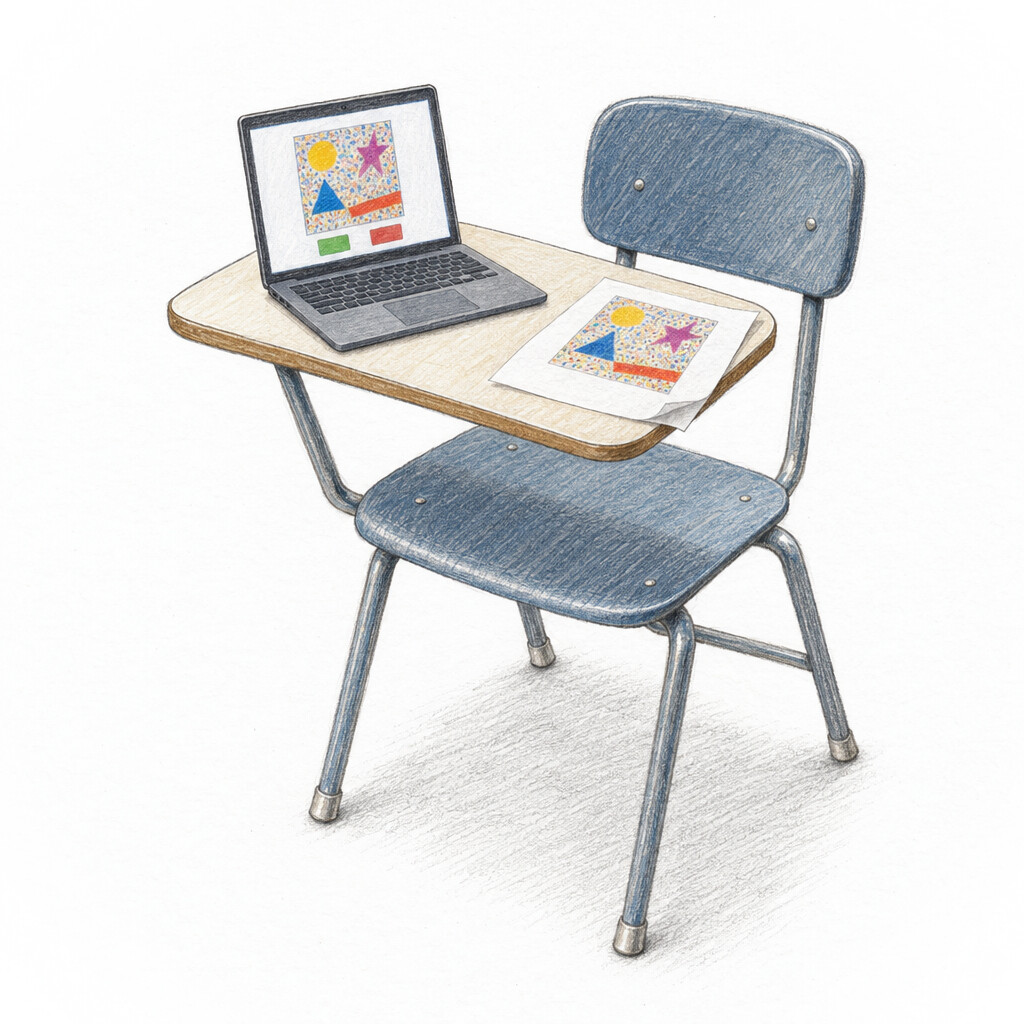
\includegraphics[width=0.5\textwidth]{figures/cover.jpg}\par\vspace{0.3em}}{}
{\itshape\fontsize{14pt}{17pt}\selectfont\color{acpink} No Paint in classrooms, two weeks on}\par
\vspace{0.5em}
{\small\color{acgray} \href{https://prompt.ac/@jeffrey}{@jeffrey} \,$\cdot$\, \ac{} \,$\cdot$\, ORCID \href{https://orcid.org/0009-0007-4460-4913}{0009-0007-4460-4913} \,$\cdot$\, 16 November 2026}\par
\vspace{0.55em}
{\color{acpink}\rule{\textwidth}{1.2pt}}
\vspace{0.4em}
\end{center}

\begin{quote}
\small\noindent\textbf{Abstract.}
On 4 November an earlier paper traced 331 paintings, saved in two school mornings with the 2016 game No Paint, to students in Lima. It left three questions open: how the classes found the site, whether they would come back, and who was teaching. Twelve days later the first two have answers. Google search carried the arrivals: 149 clicks on 3 and 4 November, 179 of the site's 203 search clicks from Peru, where nine in ten people shown the result clicked it. The classes came back. 124 paintings arrived between 10:05 and 13:00 Lima time on Monday 16 November, and 92 more on 10 and 11 November fell in a different window, 00:41 to 07:37 UTC, which is either a school morning in East or Southeast Asia or an evening in the Americas. The visit counter saw almost none of it: 124 saves came from 14 recorded visits. The third question is still open. The teacher form was opened 18 times and sent none.
\end{quote}
\vspace{0.3em}
}]

\section{Introduction}

No Paint is a painting game from 2016~\cite{scudder2016nopaint}. A painting grows one proposed mark at a time, and the player answers \emph{Paint} or \emph{No}. Its 2021 build still runs at \texttt{nopaint.art}, and saves each finished painting through its own endpoint.

The first paper, \emph{Who Is Painting}~\cite{scudder2026whoispainting}, followed a spike in that endpoint. On 3 and 4 November, 331 paintings arrived in four blocks of about one class period each, at 8:15 and 11:30 in Lima. Of the uploads still in the access log, all came from Peruvian networks and eight came from one school. It ended with three open questions:

\begin{enumerate}
\item How did the visitors find the site: Google search, Google Discover, or something else?
\item Was this a single lesson, or a class that would come back?
\item Who is the teacher?
\end{enumerate}

This paper, \emph{Who Is Still No Painting?}, reports what twelve more days of data say about each. The title keeps the game's name in the question: the players are still making No Paintings. It uses only aggregate counts. It names no school and no person, and it holds no painting codes or network addresses.

\section{Instruments}

Four reads were made on 16 November 2026.

\begin{itemize}
\item \textbf{Classic save counts.} The No Paint report counts saves by time, from the endpoint's database. Run over 840 hours it gives saves per UTC day. Run with a short window and an end time it gives the saves in that window, with the first and last save times. Its output holds counts and times only.
\item \textbf{Search Console}~\cite{google2026performance}, for \texttt{nopaint.art}, by date and by country. Google's data ends two days back, on 14 November.
\item \textbf{Daily visits}, from the first-party visit collector, which removes automated traffic. It cannot see the 2021 game's saves; the first paper explains why.
\item \textbf{App Store downloads} for the No Paint app on iPhone and iPad.
\end{itemize}

One instrument from the first paper was not used. The server's access log rolls over in under three days, so the network attribution that placed the first classes in Peru was not run for the later days. Every location in this paper after 4 November is therefore inferred from clock time and search country, not from networks.

\section{How they found it}

Table~\ref{tab:search} answers the first question. On 3 and 4 November, Google search sent \texttt{nopaint.art} 149 clicks from 223 impressions; on the fifteen days before, it sent 17 from 464. Two in three people shown the result clicked it. Peru accounts for 179 of the site's 203 clicks in the period, at a click-through rate of 90\%. In the United States, where the site was shown about as often, 5\% clicked.

\begin{table}[t]
\centering
\caption{Google search for \texttt{nopaint.art}. Days are Google's.}
\label{tab:search}
{\tbl
\begin{tabularx}{\columnwidth}{|Y|r|r|}
\hl{3}
\thead{acdark}{Days} & \thead{acpink}{Clicks} & \thead{acdark}{Shown}\\ \hl{3}
\rowcolor{acblue!8} 19 Oct to 2 Nov (15 days) & 17 & 464\\ \hl{3}
\rowcolor{acpink!10} 3 Nov & 75 & 114\\ \hl{3}
\rowcolor{acpink!10} 4 Nov & 74 & 109\\ \hl{3}
\rowcolor{acblue!8} 5 Nov & 13 & 67\\ \hl{3}
\rowcolor{acblue!8} 6 to 14 Nov (9 days) & 24 & 281\\ \hl{3}
\thead{acdark}{Country, 10 Oct to 14 Nov} & \thead{acpink}{Clicks} & \thead{acdark}{Shown}\\ \hl{3}
\rowcolor{acpink!10} Peru & 179 & 198\\ \hl{3}
\rowcolor{acblue!8} United States & 11 & 218\\ \hl{3}
\rowcolor{acblue!8} United Kingdom & 4 & 38\\ \hl{3}
\rowcolor{acblue!8} All others & 9 & 581\\ \hl{3}
\end{tabularx}}
\end{table}

The query was the name. ``no paint'' drew 147 clicks, ``nopaint'' 27 and ``no.paint'' 16. A click-through rate that high means people typing a name they had been given, which fits a teacher writing ``no paint'' on the board. Discover, the open alternative in the first paper, is not needed to explain it.

\section{The classes came back}

Figure~\ref{fig:days} shows saves per day for four weeks. Outside class days the game sees three to ten paintings a day. Five days stand far above that: 3 and 4 November, which the first paper studied, then 10, 11 and 16 November.

\begin{figure}[t]
\centering
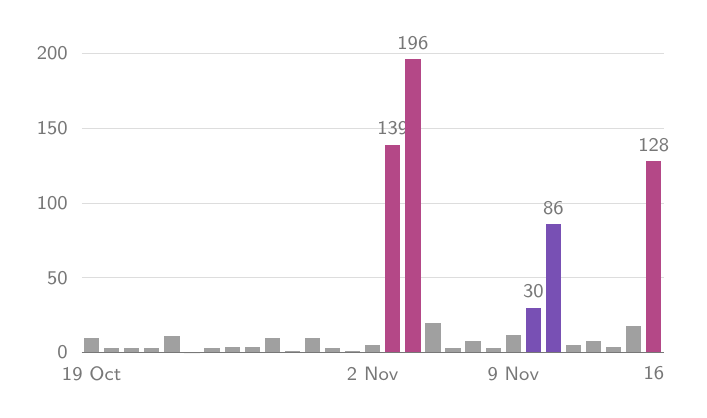
\begin{tikzpicture}[x=0.255cm,y=0.019cm]
  \foreach \y in {0,50,100,150,200} {
    \draw[acgray!25, line width=0.3pt] (0,\y) -- (29,\y);
    \node[tag, anchor=east] at (-0.2,\y) {\y};
  }
  \foreach \i/\n in {0/10,1/3,2/3,3/3,4/11,5/0,6/3,7/4,8/4,9/10,10/1,11/10,12/3,13/1,14/5,17/20,18/3,19/8,20/3,21/12,24/5,25/8,26/4,27/18} {
    \fill[acgray!70] (\i+0.12,0) rectangle (\i+0.88,\n);
  }
  \foreach \i/\n in {15/139,16/196,28/128} {
    \fill[acpink] (\i+0.12,0) rectangle (\i+0.88,\n);
    \node[tag, anchor=south] at (\i+0.5,\n) {\n};
  }
  \foreach \i/\n in {22/30,23/86} {
    \fill[acpurple] (\i+0.12,0) rectangle (\i+0.88,\n);
    \node[tag, anchor=south] at (\i+0.5,\n) {\n};
  }
  \draw[acgray, line width=0.4pt] (0,0) -- (29,0);
  \node[tag, anchor=north] at (0.5,-3) {19 Oct};
  \node[tag, anchor=north] at (14.5,-3) {2 Nov};
  \node[tag, anchor=north] at (21.5,-3) {9 Nov};
  \node[tag, anchor=north] at (28.5,-3) {16};
\end{tikzpicture}
\caption{Paintings saved with \emph{Done} in the 2021 No Paint, per UTC day, 19 October to 16 November 2026 (16 November to 21:41 UTC). Pink: days whose saves fall in Lima's school morning. Purple: days whose saves fall between 00:41 and 07:37 UTC.}
\label{fig:days}
\end{figure}

Table~\ref{tab:windows} splits the three new days into windows. Monday 16 November is the clearest. 124 of its 128 saves arrived in one block, from 15:05 to 17:59 UTC, which is 10:05 to 12:59 in Lima. That is a late-morning class period, like the 11:30 blocks of the first week, and the search country makes Lima the likely place.

\begin{table}[t]
\centering
\caption{Saves on the three new class days, by UTC window. Lima is UTC$-$5.}
\label{tab:windows}
{\tbl
\begin{tabularx}{\columnwidth}{|l|Y|r|}
\hl{3}
\thead{acdark}{Day} & \thead{acdark}{Window, UTC (first--last save)} & \thead{acpink}{Saves}\\ \hl{3}
\rowcolor{acpurple!10} Tue 10 & 02:25--07:36 & 15\\ \hl{3}
\rowcolor{acblue!6} Tue 10 & 13:44--16:49 & 6\\ \hl{3}
\rowcolor{acblue!6} Tue 10 & after 18:00 & 9\\ \hl{3}
\rowcolor{acpurple!10} Wed 11 & 00:41--05:59 & 77\\ \hl{3}
\rowcolor{acblue!6} Wed 11 & 06:06--07:18 & 3\\ \hl{3}
\rowcolor{acblue!6} Wed 11 & 13:15--14:35, 22:43--22:49 & 6\\ \hl{3}
\rowcolor{acblue!6} Mon 16 & 13:24--14:28 & 3\\ \hl{3}
\rowcolor{acpink!10} Mon 16 & 15:05--17:59 & 124\\ \hl{3}
\rowcolor{acblue!6} Mon 16 & 18:03 & 1\\ \hl{3}
\end{tabularx}}
\end{table}

\subsection{A second window}

Tuesday 10 and Wednesday 11 November look different. Their large blocks fall between 00:41 and 07:37 UTC: 15 saves on the 10th and 77 on the 11th. In Lima that is 19:41 to 02:37, the evening and the middle of the night. There are two ways to read it.

\begin{itemize}
\item \textbf{A class elsewhere.} The same window is 07:41 to 14:37 at UTC$+$7, 08:41 to 15:37 at UTC$+$8 and 09:41 to 16:37 at UTC$+$9, a school day in much of East and Southeast Asia. Tuesday and Wednesday match the weekdays of the first Lima classes, which would be a coincidence.
\item \textbf{Homework in the Americas.} 77 paintings in five evening hours could be many students finishing an assignment at home.
\end{itemize}

The data cannot choose between them. The access log that would show the networks had rolled away before it was read, and Search Console shows no second country with more than four clicks. One detail leans toward a class: the teacher form was opened twice inside the 10 November window, and a student doing homework has no reason to open a form written for teachers.

\section{What the visit counter misses}

The first paper's wrong turn was asking the visit counter about saves it could not see. Two weeks later the gap is wider, because a class keeps one page open and saves many paintings from it.

\begin{table}[t]
\centering
\caption{Saves beside recorded visits to \texttt{nopaint.art}. The 16 November row is the three-hour class block.}
\label{tab:gap}
{\tbl
\begin{tabularx}{\columnwidth}{|Y|r|r|}
\hl{3}
\thead{acdark}{Period} & \thead{acdark}{Visits} & \thead{acpink}{Saves}\\ \hl{3}
\rowcolor{acpink!10} 3 Nov & 344 & 139\\ \hl{3}
\rowcolor{acpink!10} 4 Nov & 452 & 196\\ \hl{3}
\rowcolor{acpurple!10} 10 Nov & 42 & 30\\ \hl{3}
\rowcolor{acpurple!10} 11 Nov & 32 & 86\\ \hl{3}
\rowcolor{acpink!10} 16 Nov, 15:00--18:00 UTC & 14 & 124\\ \hl{3}
\end{tabularx}}
\end{table}

Table~\ref{tab:gap} shows the change. In the first week visits outnumbered saves: students arrived from Google one by one. By the third week a class made 124 paintings in 14 recorded visits. Daily visits to \texttt{nopaint.art} fell from 85 a day over 2 to 15 November to 28 a day in the last week of that span, while the classes went on. A report built on visits alone would say the classroom use had ended.

\section{Teachers, sticker and app}

\textbf{The teacher form} added on 4 November has been opened 18 times and sent none. It asks for several fields. The two openings during the 10 November window are the closest the data comes to a teacher.

\textbf{The sticker test} on the title screen points half of visitors at the AI studio \texttt{notepaint.art} and half at \texttt{aesthetic.computer}. The Notepaint arm was opened by 117 of the 717 visits shown it, 16\%, and 50 of those made something. The \ac{} arm was opened by none of 65. For a student in a lesson, a link that leaves the lesson is mostly ignored.

\textbf{The iPhone and iPad app} had 40 first-time downloads in 30 days, about one a day with no rise on class days. The classes use the web game.

\section{Ethics, privacy, limitations}

The makers are probably minors, in class, who did not choose to be studied~\cite{livingstone2019children}. This paper keeps to counts and times. It shows no paintings, names no school, and ran no network attribution after 4 November.

The limits are these. Locations after 4 November are inferred from clock time and search country. The second window has two readings, and the data does not decide between them. A UTC day can hold more than one group, so per-day counts mix them; the window table separates them only as far as the gaps between saves allow. Visits are page visits, not people. 16 November is a partial day.

\section{What would answer the rest}

\begin{enumerate}
\item \textbf{Ask the teacher with one field.} A single email field, in Spanish first, in place of the current form. Eighteen openings and no sends say the form is the obstacle.
\item \textbf{Count saves by hour in the daily report.} The windows in Table~\ref{tab:windows} took eleven separate reads. An hourly series would show each class as it happens.
\item \textbf{Keep a daily network summary.} Network owner names and counts only, never addresses, written once a day before the log rolls. That alone would settle the second window.
\end{enumerate}

\section{Conclusion}

The first paper found a classroom. This one finds that the classroom came back, and that there may be a second. Students in Lima reach No Paint by typing its name into Google, and on Monday 16 November one class made 124 paintings in under three hours. A second burst of 92 paintings, on a Tuesday and a Wednesday, fell in the early hours UTC, in someone's school morning or someone's evening. Through all of it, the newest instrument, the visit counter, saw the least. The question with the most value is still the one only a teacher can answer.

{\footnotesize
\begin{thebibliography}{9}\setlength{\itemsep}{1pt}
\bibitem{scudder2016nopaint} J.~Scudder, A.~Freundlich, E.~Fleck, C.~Klein et al. \emph{No Paint}. 2016. \url{https://nopaint.art}
\bibitem{scudder2026whoispainting} @jeffrey. \emph{Who Is Painting: An investigation of 331 No Paint paintings that arrived in two school mornings}. \ac{} papers, 4 November 2026. \url{https://papers.aesthetic.computer}
\bibitem{google2026performance} Google. \emph{Performance report (Search results)}. Search Console Help, 2026. \url{https://support.google.com/webmasters/answer/7576553}
\bibitem{livingstone2019children} S.~Livingstone, M.~Stoilova, R.~Nandagiri. \emph{Children's data and privacy online: Growing up in a digital age}. LSE, 2019.
\end{thebibliography}}

\end{document}
